% Chapter Template
\setstretch{1}
\chapter{Industry Engagement and Community Based Research}\thispagestyle{empty} % Main chapter title
% and Design Research: Community Collaboration in Software Development
\label{Chapter3} % Change X to a consecutive number; for referencing this chapter elsewhere, use \ref{ChapterX}

\lhead{Chapter 3. \emph{Industry Engagement and Community Based Research}} % Change X to a consecutive number; this is for the header on each page - perhaps a shortened title

\setstretch{2}
%-----------------------------------
%	Software Design for Game Jam
%-----------------------------------
\section{Theory and Politics}
Cixous' "Laugh of the Medusa" predates the computer age but perfectly and predictably describes the opportunity present in programming - which is a form of writing - within "Laugh of the Medusa":
\begin{quote}
"Write, let no one hold you back, let nothing stop you: not man; not the imbecilic capitalist machinery, in which publishing houses are the crafty, obsequious relayers of imperatives handed down by an economy that works against us and off our backs; and not yourself." 
\textit{\parencite{cixous}}
\end{quote}

In this passage, Cixous chides her readers for not giving themselves the permission to write, because writing is reserved for those who might be published. This is similar to game-makers who might not produce, merely because the engines are closed, or distribution unlikely. Women have a long history in technology.
Ada Lovelace, daughter of Lord Byron, has been identified as the first programmer \parencite{plant}. The ability to put rules in order, to work backwards and forwards from a desired result all along the path of the machines, is a characteristic much sought for in both programmers and game designers. Both roles are responsible for rule systems that will dictate a predictable result.

In a straightforward way, ladies may not possess uncomplicated positions of economic advantage within a patriarchy: to do so would be to "have it all," a famously complex desire which is reanalyzed every year in popular press, most recently by Anne-Marie Slaughter in \textit{The Atlantic} \parencite{slaughter}. The balancing factor is housework and the social expectation of family, which still places a gendered burden on women to produce both children and home. This system of expectations, divided between household and the potential for earned income, re-creates itself in each new trade as it arrives, in fields as far apart as World War II factories \parencite{summerfield}, Victorian mills \parencite{baskerville}, and lately, code factories in Manhattan and San Francisco \parencite{newdomestic}. Computers have quickly become a good job with a good chance to better one's life, and just as quickly have moved from being women's work to being a heavily masculinized field \parencite{ensmenger}. This is unfortunate, as it is presently popular to assert that in the future, there will be two types of lives:

\begin{quote}
"...those who tell computers what to do, and those who're told by computers what to do."
\textit{Marc Andreesen, Andreesen Horrowitz 2012.}
\end{quote}

Within such a system, people discouraged from understanding technical roles, their uses and disuses, could then be expected to be mainly among those being told what to do. This does not seem to be a pleasant future, inclusive and positive for all people, and as such, perhaps the vision could be broadened.

Computers are a tool, and the way that the tool is presented, held, and used, dictates the results. A computer - a machine for automating an interaction - can be made simpler or more complex to use. The device may be changed to an amplifier of force, made more opaque, or made clearer for those who choose not to learn to code but can still understand systems of logic. "If this then that" is not a complex instruction set. The complex instruction sets should, rather than being encouraged to control people, be developed to be under the control of people.

screenPerfect has been designed to present the idea that a simpler system will result in a more diverse body of work. It dictates nothing whatsoever about content, presenting instead a simple system of switches that permits the author the broadest possible control over simplified interaction sets. It is implied that these interactions will lead to a coherent narrative but it does not dictate what content an artist might use. The voice of the artist is brought to the forefront of the work, rather than the voice of technology.

By simplifying the process of game design and displacing its nexus from the computer to other design tools, technology is repurposed to be one tool among many. This displaces technology's primary position and refocuses the work on the intent of the artist. This is an implicit system of resistance to the narrative of technology: people can once again tell computers what to do, and extend themselves via their tools.

\section{Cixous, Embodiment, and the Game Jam}

Many of the participants of the game jam produced, with the simple yet powerful tools provided, narratives centered on their own embodied or disembodied experience. The only group to resist doing this were the younger OCADu students who came to the jam via a game design practice, rather than a filmmaking, animation, photographic or other digital interest.

Of the games produced and finished, \textit{PornGame} by Max Lander is directly about the experience of sexuality as it applies to a machine. Grimoire is about a loss of personal agency following the finding of a "grimoire" or textbook. \textit{Kill Fuck Marry} was about bad decisions when it came to dating and sex, \textit{OM} about a practice of embodied mindfulness, and \textit{Cyborg Goddess} went straight to Donna Haraway's "Cyborg Manifesto" in a literal interpretation. \textit{Glitch.95}, though mainly interested in the glitch aesthetic, is a depiction of the beginnings of an internet relationship. \textit{Puppet Story} is about a genderless creature coming to life, Pinocchio-esque - or perhaps more Galatea, though that is projection.

This is simply an observation but a comparatively high number of personal and body-centric stories came from this jam, which was nominally about the use of a tool to express a new format of interaction software. This seems tied to Cixous' assertion that "You can't talk about \textit{a} female sexuality" and her immediate follow-up that "time and again I ... could burst forth with forms much more beautiful than those which are put up in frames and sold for a stinking fortune" \parencite{cixous}. This is the core of what games critics are discussing when independent games, or new art forms of any type, are being spoken about publicly - the potential expression outside commercial benefit. Cixous's conception of masturbation and writing as a unified activity practiced in secret can be easily associated to the idea of imposter syndrome, the thought that one could not possibly be "good enough" to break into a creative or high-level industry \parencite{imposter}. 

Imposter syndrome is a major problem in the technology industry, and in games even moreso: because code is a high-level creative practice, with a great deal of material reward when done properly, and games are similar, the stakes are high. I have conflated games and code because both are systems of organized rules: game design is a type of code, where one purses conditioned response and engagement through good user experience design. It is easy to back off from both practices or to pursue them exclusively as a hobby, rather than believe in them as a trade. Does one wish to join the commercial order? Is it necessary to be validated, to have commercial success, or is it simply another demand on the work, that the work sell to prove that it is fundamentally worthwhile? These questions are outside the scope of this paper, although my personal opinion is in line with Cixous: whether the money follows or not, a plurality of voices in any creative practice is important for its own sake.

Cixous' throwaway line, of "arid millenial ground to break" seems especially poignant in light of the generational nickname of the jam participants. 


\section{Industry Engagement}
\subsection{Game Jams, A Design Method}
A game jam is a variant on the hackathon, which is a type of prolonged effort at taking an idea from concept to finished product in a limited period of time. Game jams and hackathons are both derived from the design charette or parallel prototyping process \parencite{martin}, a method in which participants rapidly prototype a design idea over a short, intense period of time. Charettes stem from the architecture field, and benefit from the idea of a concentrated sprint of effort to complete a given project in a narrow window, thus preventing the project from creeping too far out of scope. A jam - or hackathon - gives registered participants a common area and space to set up their own equipment and supplies, and a theme. The group members come to the event with an idea and possibly some resources - video files, sound capability and so on - and use the jam time to assemble a game.

Generally, a game jam will produce a panoply of small game ideas with fleshed-out mechanics but simple art and sound design in order to demonstrate a possible path forward for a device or piece of software, which will then be polished at a later date, and presented to the indie community either online or at a social event. Sometimes these works will then go on to be finished commercial products, or are intended for further consumption at major conferences such as Indiecade or the Game Developer's Conference, GDC. These conferences can further the careers of the developers by providing access to funding bodies and publishing houses (whether traditional or online), or in Ontario, the Ontario Media Development Corporation. Other funding sources can include research groups, via research funding bodies. By framing game jam development as research, participants can be released from the need to make commercially appealing works. In the case of Dames Making Games and screenPerfect, funding came from the Feminists in Games project, headed by Jen Jenson of York University, and GRAND FRAGG, a research project dedicated to expanding the diversity of voices represented in gaming. This research funding supported the research goals of this collaboration led by Professor Emma Westecott at the game::play Lab.

Game jams can be time consuming to prepare, as they involve a great deal of communication on the part of the organizers. In order to run a jam, one must open the application period well enough in advance to ensure a large cohort of skilled participants who are likely to be interested in producing content with the available tools, or interested in exploring new tools on offer. Typically, jam attendees have a theme suggested - for example, "Mother May I" or "Snacktember" jams organized by Dames Making Games - and then participants bring their own preferred technology to produce a fast prototype over a weekend.

\subsection{Dames Making Games and Game Jams}
\begin{quote}
Dames Making Games (DMG Toronto) is a non-profit community organization based in Toronto dedicated to supporting dames interested in making, playing, and changing games. In short, we want to build an \textbf{inclusive} and \textbf{engaged} local community of game-makers. Our community isn't women only but it is women-driven.
\textit{from the DMG.to website, accessed November 27, 2013}
\end{quote}

Dames Making Games (DMG) is a community group in Toronto that work to promote women in video games. They have been funded in part by FiG (\url{http://www.feministsingames.com}) and in part by member donations. I am a founding director and advising director with the organization, which has given me ready access to a test audience for my ideas with regards to development tools. DMG uses the game jam method to introduce women and allies to simple game development tools. This provides a straightforward introduction to concepts of computer logic and programming for some people, to video game art development for others, and video game sound production for still others. Some develop system mechanics, some design whole levels or game narratives. 

The point of DMG is to promote access to this field to people other than the 18-to-35 year old males who form the primary demographic for the video game industry \parencite{esa, igda}, in the hopes that a diverse population of game makers will produce a diverse population of games. DMG is interested in screenPerfect as it provides an underlying template for a game-making system that might be easier for newcomers to use than other freely available game engines.

\subsection{Bento Box-Miso}
Game jams require both space and people who are interested in working on games. A themed game jam, such as No Jam 2, which was designed to test specific software, requires a specific audience and support. In order to access that space and community, I worked with the Bento Box-Miso co-working facility in Toronto, with OCADu's game:play lab and Emma Westecott, and with Bento Box-Miso, a development company that runs Bento Box-Miso as a not for profit co-working facility.

Bento Box-Miso is a not-for-profit community coworking facility that serves as home for both Bento Box-Miso, a local development hub, and the Dames Making Games. It is also the hub of a great deal of Toronto's independent game development community. Bento Box-Miso offers professional support and development advice to game developers. I felt there was a good match between their professional skillset and my research interests. DMG regularly run a jam in November and felt that screenPerfect - new software designed to be usable in a short time frame to people with extant skills - would be a good match for the audience associated with the organization. 

Bento Box-Miso was also at the time seeking an engine that could display the capabilities of their new programming language, Daimio, which offers users the ability to reprogram work on the fly in the browser without being a trusted network source. Therefore, I accepted their help and their offer of hosting the jam in return for giving them permission to fork - copy, reproduce, and extend - my engine under their name. 

As a pair, Dann Toliver - architect of Daimio - and I worked together to clean screenPerfect to speak to the Daimio dataflow language. Bento Box-Miso then released a refactored version of the code in time for No Jam 2, so that our participants could get a clean version of the software to work with. This was challenging for me, as it involved a great deal of trust and moved the software away from how I had initially envisioned the user interface (UI). In particular, we needed to scrap an early idea for a branched narrative "tree" display similar to that of the Twine engine, which was not included, although it had been planned all along (Figure 3.1).

\newpage
\begin{figure}[h!]
 \centering
 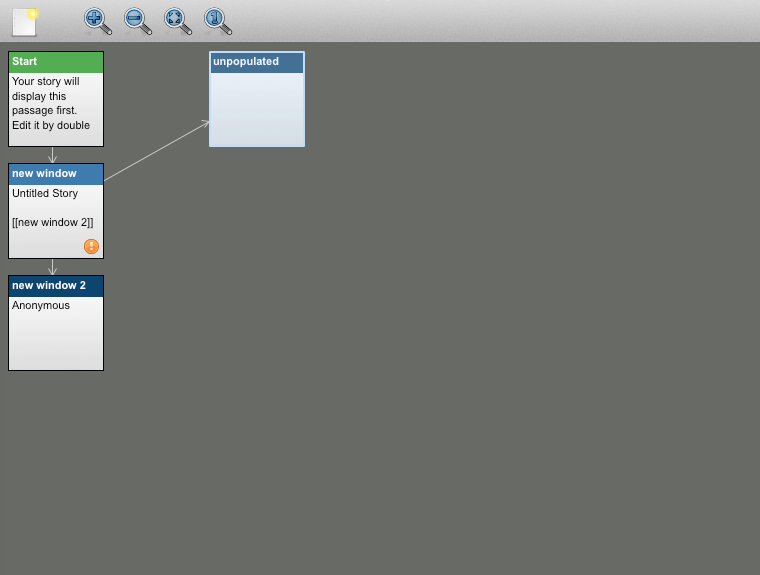
\includegraphics[width=\textwidth]{twineNodeTree}
 \caption{A branched tree of rooms from Twine.}
\end{figure}
\newpage

\subsection{No Jam 2: Video Video}
DMG have a great deal of experience running jams. In addition to a skilled community, the ongoing success of research in the community is dependent on participation by community members' voluntary engagement in participatory research. The premise of DMG is that people learn well by doing something new in a supportive environment and that they can carry the experience of a supportive learning environment forward to effect real change in the game development landscape. game::play Lab is researching the outcomes and process of this type of development practice. By partnering with DMG, I gained ready access to their community and they gained access to my software. One of the most common difficulties with game jams is that the short timeframe can cause a lot of frustration to new non-programmers: they spend a lot of time wrestling with tools, rather than generating the content of their games. This is a theme that came up again and again in research interviews, most notably and clearly presented in Appendix A's DVD support by Team Grimoire - Katie Foster and Mikayla Carson:

\begin{quote}
"I've come to jams three times now and I never do it very well... the new tool caused me to change my concept and execution but not by much. It's learning on the first day if I can make my idea work with that tool and then teaching myself that tool, because usually I have no idea how to use it.... I like the constraints that have been put on the project, since it's made me pursue new things I'd never pursue. ... It's like five rooms, they all hook straight to the next one, I'm not intimidated about putting it into the tool. ... that's what's so awesome, I'm so used to having to learn ALL new skills, every time I jam, and then I get really frustrated and I don't want to do it any more, so this time I'm like 'I know how to do all this stuff already.'"
\end{quote}

The reduction in technical barriers to entry resulted in five complete games coming out of the No Jam process, one of which was exhibited at the Art Gallery of Ontario.

After we received No Jam applications, we went through them to choose participants who seemed interested the theme and the software restrictions, sent out acceptances, ordered food, and set the dates. Applicants were provided diaries to record their working process over the course of the week. The first weekend of the jam consisted of workshops from a variety of specialists to provide direction in how to think about the software and the jam process as research.

The applicants were then sent home for a week to work on their video projects. They were asked to document their ongoing process with one another on a private Google Group. Most participants ignored this request, which left us with relatively little online material.

On the actual weekend, we asked that participants arrive with the majority of their video content and design prepared. There were uneven responses to this request, which strongly affected the ability of participants to produce a finished game by the end of the weekend. I interviewed each group early in the process and then later polled them with informal questions regarding their experience with the software. The interviews are documented in my electronic support materials in named files. During interviews, I asked participants about their background, what they expected from a game jam, their previous experience in game or media design. I also asked whether they found the restrictions of working with the screenPerfect software package useful, damaging, easy, or difficult. The main responses of interest were not about the software at all, although Mikayla Carson clearly stated that as a filmmaker she found screenPerfect much less frustrating than traditional game engines. The responses of most interest involved how people think about producing media, their frustrations with traditional computer work, and their experience with collaborative game practice.

I asked each group to name themselves, talk about their background, and tell me what they expected out of a game jam. Then, if appropriate, I asked what their experience with the software was and how it compared to other game-making engines and software. The interviews with each group proved diverse. Responses are recorded on my electronic supporting materials in the appendices, under the folder "Game Jam Interviews."

The group experience with the software proved interesting. Accomplished filmmakers had a better time with it but the most surprising response was from young, self-identified gamemakers, who rather than exploring what was possible within the context of the software tools, decided instead to try to use them to reproduce existing game types, many of which were totally incompatible with the software design. Of particular interest was the group who tried to reproduce a classic Japanese roleplaying game within the context of video: this did not work so well. The group continued to work on their design even after it became apparent it was unlikely to go well. The game itself remains unfinished but deserves mention as the most unique and possibly stubborn effort.

Despite this, No Jam was a success, with nine groups producing diverse works on ideas such as how to express a practice of mindfulness, how to work with pornography in a way that forces the viewer to interact with what's happening on screen, exploring systematic violence against women, exploring narratives of imprisonment, magic, and in one unique case, permitting a puppet to escape a toy box. 

In setting up No Jam, we did present at least one workshop on the importance of personal narrative in producing creative work, which may have influenced the results. Game jammers mostly described their interest in producing work that was finished. No Jam resulted in at least five "finished" works, which have since been included in several exhibitions around the city, including the December and January Toronto Long Winter series. The finished works can be found on the supporting materials DVD under the folder "screenPerfect games."